\subsection{Dirac-Notation von Vektoren in der Quantenmechanik}
In der Quantenmechanik werden Vektoren üblicherweise mit folgendem Symbol notiert:
\cf{
    \cket{v}\quad\text{("ket"-Vektor)}
}
Der adjungierte Vektor wird wie folgt geschrieben: \cf{\cket{v}^\dagger = \cbra{v}\quad\text{("bra"-Vektor)}}
Das Skalarprodukt zweier Vektoren \ket{v} und \ket{w} ergibt sich aus der Verschmelzung von \it{bra} und \it{ket} zu: 
    \cf{
    \left\langle v|w\right\rangle 
}
Zwischen \it{bra} und \it{ket} kann auch ein Operator stehen:
\cf{
    \left\langle v|A|w\right\rangle
}
Dies ist das Skalarprodukt von \ket{v} mit dem Vektor \f{A\cket{w}} bzw. das Skalarprodukt von \f{A^\dagger\cket{v}} mit \ket{w}: 
\cf{(A^\dagger\cket{v})^\dagger = \cket{v}^\dagger(A^\dagger)^\dagger = \cbra{v}A}
Neben dem Skalarprodukt gibt es auch ein "äußeres Produkt", bei dem \it{bra} und \it{ket} in umgekehrter Reihenfolge erscheinen:
\cf{
    \cket{v}\cbra{w}
}
Dies ist ein Operator, dessen Wirkung auf einen Vektor \ket{u} naheliegenderweise wie folgt definiert ist (wobei die runden Klammern weggelassen werden können):
\cf{
    (\cket{v}\cbra{w})\cket{u} = \cket{v}(\left\langle w|u\right\rangle) = \cket{v}\left\langle w|u\right\rangle
}
Von Mathematikern wird die Schreibweise manchmal kritisiert, da es vermeintlich zu Zweideutigkeiten kommen kann, z.B. \f{\cket{v}\skal{w}{u}} kann bedeuten: (1) Vektor \ket{v} multipliziert mit Skalarprodukt \f{\skal{w}{u}}, oder (2) die Wirkung des Operators \ket{v}\bra{w} auf den Vektor \ket{u}.\\
In der Praxis ist dies kein Problem (und erlaubt beim Aufschreiben von Formeln größere Flexibilität), da beide Deutungen dasselbe Ergebnis liefern.

\subsubsection*{Beispiele für Dirac-Notation}
Zweidimensionaler Vektorraum mit Basis \f{(\cket{0},\cket{1})}:
\begin{itemize}
    \item \f{A = \cket{1}\cbra{0} = \begin{pmatrix}0&0\\1&0\end{pmatrix}}\\
        \f{A\cket{0} = \cket{1}\underbrace{\skal{0}{0}}_{=1} = \cket{1}\qquad \begin{pmatrix}
        0&0\\1&0
        \end{pmatrix}\begin{pmatrix}
        1\\0
        \end{pmatrix}=\begin{pmatrix}
        0\\1
        \end{pmatrix} }\\
        \f{A\cket{1} = \cket{1}\underbrace{\skal{0}{1}}_{=0} = 0\qquad\ \ \begin{pmatrix}
        0&0\\1&0
        \end{pmatrix}\begin{pmatrix}
        0\\1
        \end{pmatrix}=\begin{pmatrix}
        0\\0
        \end{pmatrix} }
    \item \f{B = b_{00}\cket{0}\cbra{0}+b_{01}\cket{0}\cbra{1}+b_{10}\cket{1}\cbra{0}+b_{11}\cket{1}\cbra{1} = \matr{b_{00}&b_{01}\\b_{10}&b_{11}}}\\
    \f{\left\langle 0|B|0\right\rangle = b_{00}\skal{0}{0}\skal{0}{0}+b_{01}\skal{0}{0}\skal{1}{0}+ b_{10}\skal{0}{1}\skal{0}{0}+b_{11}\skal{0}{1}\skal{1}{0} = b_{00}}
\end{itemize}
\f{\Rightarrow\text{ Im allgemeinen liefert }\left\langle i|B|j\right\rangle\text{ das Matrixelement von }B\text{ bzgl. der Basis }\left\{\cket{i}\right\}}.


\newpage
\subsection{Quantenmechanik von Qubits}
Ein Qubit ist ein quantenmechanisches System mit 2 verschiedenen Basiszuständen, im folgenden als \ket{0} und \ket{1} bezeichnet. Dies ist ein idealisiertes Konzept, da tatsächliche Quantensysteme (z.B. einzelne Atome) mehr als 2 (meist sogar unendlich viele) Zustände haben. Um ein Qubit zu realisieren, muss also der experimentelle Aufbau so geschickt gewählt werden, dass die überzähligen Zustände vernachlässigt werden können, z.B. wie folgt:
\begin{figure}[h!]
    \centering
    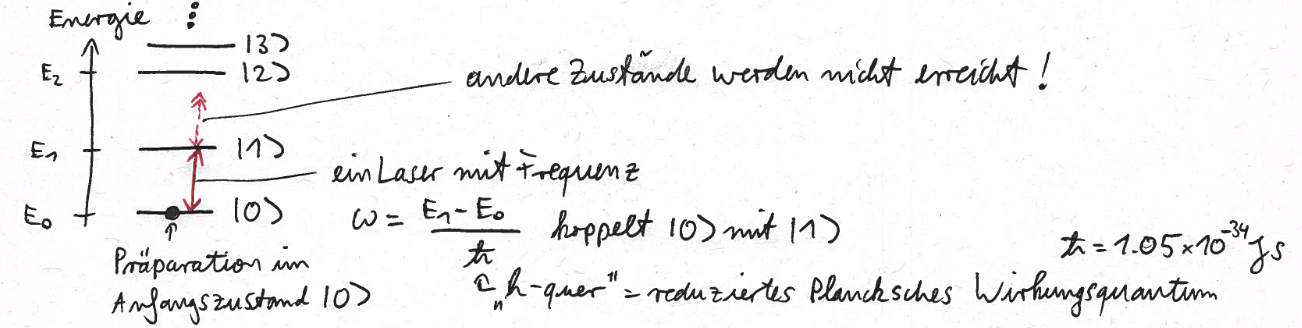
\includegraphics[width=.8\textwidth]{images/zustände.png}
\end{figure}
Mögliche Zustände des Qubits werden durch normierte Vektoren im von \ket{0} und \ket{1} aufgespannten 2-dimensionalen komplexen Vektorraum beschrieben:
\cf{
    \cket{\psi} = a_0\cket{0}+a_1\cket{1} = \matr{a_0\\a_1}\qquad a_0,a_1\in\mathbb{C}\text{ mit }|a_0|^2+|a_1|^2=1\text{ (Normierung)}
}

\subsubsection*{Messung}
Um Informationen über den Zustand des Qubits zu gewinnen, können wir eine Messung durchführen. Diese geschieht stets bezüglich einer bestimmten Orthonormalbasis, welche durch den Aufbau der Messapparatur bestimmt wird. Im Quantencomputing betrachtet man normalerweise nur Messungen bzgl. der Standardbasis (\ket{0} oder \ket{1}). Das Ergebnis der Messung ist \b{zufällig}, und zwar:
\begin{align*}
    p_0 &= |\skal{0}{\psi}|^2 = |(1,0)\matr{a_0\\a_1}|^2 = |a_0+0\cdot a_1|^2 = |a_0|^2\qquad\text{ Wahrscheinlichkeit für Ergebnis "0"}\\
    p_1 &= |\skal{1}{\psi}|^2 = |(0,1)\matr{a_0\\a_1}|^2 = |0\cdot a_0+a_1|^2 = |a_1|^2\qquad\text{ Wahrscheinlichkeit für Ergebnis "1"}
\end{align*}

\b{Nach der Messung} befindet sich das Qubit dann in dem Zustand, der dem gemessenen Ergebnis entspricht, d.h. \f{\cket{\psi}=\cket{0}} oder \f{\cket{\psi}=\cket{1}} ("Zustandsreduktion"). Eine Messung in der \ac{qm} hat also folgende Eigenschaften:
\begin{itemize}
    \item Ergebnis ist zufällig (wobei die Wahrscheinlichkeit für die verschiedenen möglichen Ergebnisse vom Zustand \ket{\psi} abhängen)
    \item Der Zustand \ket{\psi} wird durch die Messung verändert ("Kollaps des Quantenzustands")
\end{itemize} 
\vspace{1em}
\b{Frage:} Wer oder was entscheidet, ob das Ergebnis "0" oder "1" ausgewählt wird?\\
\f{\quad\rightarrow\quad} Antwort unbekannt! ("Messproblem" in der \ac{qm})\\
\vspace{1cm}

Für eine Messung bzgl. einer beliebigen Orthonormalbasis (\ket{v_1},\ket{v_2}) mit \f{|\skal{v_i}{v_j}|=\delta_{ij}} gilt entsprechend:
\cf{
    p_{v_i} = |\skal{v_i}{\psi}|^2\quad\text{Wahrscheinlichkeit für Messergebnis "}v_i\text{" } (i = 1,2)
}
Die Messung geht einer mit der entsprechenden Reduktion des Zustands:
\cf{
    \underbrace{\cket{\psi}}_{\text{Zustand vor der Messung}}\rightarrow\underbrace{\cket{v_i}}_{\text{Zustand nach der Messung mit Ergebnis "}v_i\text{" (i=1\text{ oder }2)}}
}

\subsubsection*{Dichteoperator und Invarianz bzgl. globaler Phase}
Betrachten wir einen beliebigen Zustand \ket{\psi} eines Qubits sowie \f{\cket{\psi^\prime}=e^{i\varphi}\cket{\psi}} mit \f{\varphi\in\mathbb{R}}, dann gilt:
\cf{
    p_{v_i}^\prime = |\skal{v_i}{\psi^\prime}|^2 = |e^{i\varphi}\skal{v_i}{\psi}|^2 = \underbrace{|e^{i\varphi}|^2}_{=1}\underbrace{|\skal{v_i}{\psi}|^2}_{=p_{v_i}} = p_{v_i}
}
Dies zeigt, dass \ket{\psi} und \ket{\psi^\prime} dieselbe Wahrscheinlichkeit für Messung in beliebiger Basis liefern!\\
Wir definieren nun den zu \ket{\psi} gehörigen Operator ("Dichteoperator" oder "Dichtematrix"):
\cf{
    \varrho = \cket{\psi}\cbra{\psi} = \matr{a_0\\a_1}\matr{a_0^* & a_1^*} = \matr{|a_0|^2 & a_0a_1^*\\a_1a_0^* & |a_1|^2} \qquad \text{(Darstellung bzgl. Standardbasis)}
}
\b{Achtung:} Der Dichteoperator ist nicht zu verwechseln mit dem Skalarprodukt:
\cf{\skal{\psi}{\psi} = \matr{a_0^*&a_1^*}\matr{a_0\\a_1} = |a_0|^2 + |a_1|^2 \in \mathbb{C}}
Der Dichteoperator liefert eine eindeutige Beschreibung der Wahrscheinlichkeiten für Messungen in beliebiger Basis:
\cf{
    p_{v_i} = |\skal{v_i}{\psi}|^2 = \skal{v_i}{\psi} \skal{v_i}{\psi}^* = \langle v_i\underbrace{\cket{\psi}\ \cbra{\psi}}_{=\varrho}v_i\rangle = \left\langle v_i|\varrho|v_i\right\rangle
}
Insbesondere sind die zu \ket{\psi} bzw. \ket{\psi^\prime} gehörigen Dichteoperatoren identisch:
\begin{gather*}
    \cket{\psi} = \matr{a_0\\a_1}\quad,\quad\cbra{\psi}=\matr{a_0^*&a_1^*}\quad,\quad\cket{\psi^\prime}=e^{i\varphi}\matr{a_0\\a_1}=\matr{e^{i\varphi} a_0\\e^{i\varphi} a_1}\quad,\quad\cbra{\psi^\prime}=\matr{e^{-i\varphi}a_0^* & e^{-i\varphi}a_1^*}\\
    \Rightarrow \varrho^\prime = \cket{\psi^\prime}\cbra{\psi^\prime} = e^{i\varphi}\cket{\psi}\cbra{\psi}e^{-i\varphi} = \cket{\psi}\cbra{\psi} = \varrho
\end{gather*}

\subsubsection*{Zustandstomographie eines Qubits}
Können wir den Zustand eines Qubits durch Messung bestimmen? Eine einzelne Messung reicht hierfür nicht aus; wir brauchen Mittelwerte über viele Messungen, um Wahrscheinlichkeiten abschätzen zu können. Da jedoch jede Messung den Zustand eines Qubits verändert, muss nach jeder Messung das Qubit erneut im ursprünglichen Zustand präpariert werden. Um den Dichteoperator \f{\varrho=\cket{\psi}\cbra{\psi}} eines Qubits vollständig zu bestimmen, benötigen wir Messungen in 3\footnote{Warum 3? - Um die 3 Komponenten des Blochvektors zu messen.} verschiedenen Orthonormalbasen.

\subsubsection*{Bloch-Vektor}
Wir definieren folgende 3 Operatoren (so genannte "Pauli-Operatoren"):
\cf{
    X = \matr{0&1\\1&0}\quad,\quad Y=\matr{0&-i\\i&0}\quad,\quad Z=\matr{1&0\\0&-1}
}

Die Pauli-Operatoren haben folgende Eigenschaften:
\begin{itemize}
    \item Selbstadjungiert: \f{X=X^\dagger, Y=Y^\dagger, Z=Z^\dagger}
    \item Spur=null: Tr(\f{X}) \f{=} Tr(\f{Y}) \f{=} Tr(\f{Z}) \f{=0}
    \item $\begin{aligned}[t]
        & XY=iZ   && , \quad YZ=iX   && , \quad ZX=iY \\
        & YX=-iZ  && , \quad ZY=-iX  && , \quad XZ=-Y
    \end{aligned}$
    \item \f{X^2=Y^2=Z^2=\mathbb{I}}
\end{itemize}
Mit Hilfe der Pauli-Operatoren kann die Dichtematrix eines Qubits anschaulich als dreidimensionaler, reeller Vektor dargestellt werden.
\definition{Blochvektor}{
    Für normierte Zustände \f{\varrho} mit Tr(\f{\varrho}) \f{=1} ist der Blochvektor definiert als:
    \begin{equation}
        \overrightarrow{s} = \matr{s_X\\s_Y\\s_Z}\quad\text{ wobei }\qquad\begin{matrix}
            s_X = \text{Tr}(\varrho X)\\
            s_Y = \text{Tr}(\varrho Y)\\
            s_Z = \text{Tr}(\varrho Z)
        \end{matrix}
    \end{equation}
    Umgekehrt gilt:
    \begin{equation}
        \varrho = \frac{1}{2}(\mathbb{I}+s_XX+s_YY+s_ZZ)
    \end{equation}
}
\b{Beweis:}
\begin{align*}
    \text{Tr}(\varrho X) &= \frac{1}{2}(\tr{\mathbb{I}X}+ s_X\tr{XX}+s_Y\tr{YX}+s_Z\tr{ZX})\\
    &= \frac{1}{2}(\tr{X} + s_X\tr{\mathbb{I}} - is_Y\tr{Z} + is_Z\tr{Y}) \\
    &= \frac{1}{2}2s_X = s_X\qquad\checkmark\quad\text{(ebenso für \f{\tr{\varrho Y}} und \f{\tr{\varrho Z}})}\\
    \tr{\varrho} &= \frac{1}{2}\tr{\mathbb{I}} = 1\qquad\checkmark
\end{align*}
Damit ist gezeigt: (Eq. 2) erfüllt die Gleichungen (Eq. 1) und die Bedingung \f{\tr{\varrho}=1}.\\
Die Eindeutigkeit von (Eq. 2) folgt aus der linearen Unabhängigkeit der Operatoren \f{\mathbb{I}, X, Y} u. \f{Z}. \f{\square}
\vspace{0.5cm}

\begin{minipage}{.48\textwidth}
\b{Blochkugel}
\begin{center}
    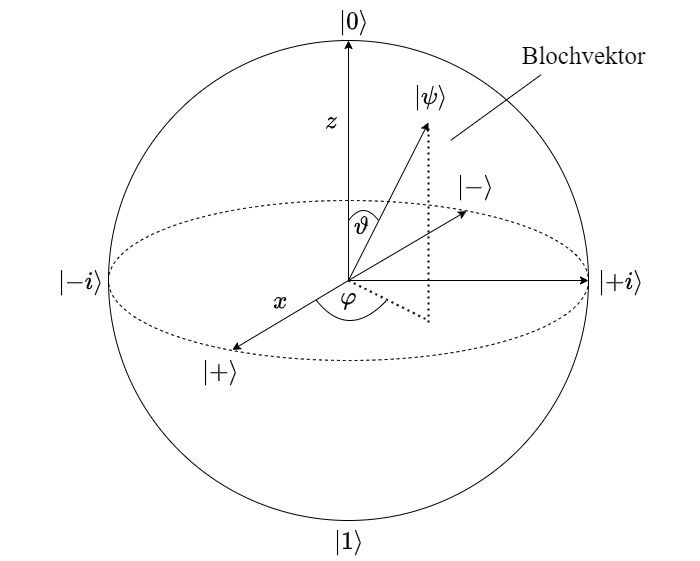
\includegraphics[width=.95\textwidth]{images/blochsphere.png}
\end{center}
\end{minipage}
\begin{minipage}{.5\textwidth}
\begin{tabular}{c|c|c}
    \toprule
    \textbf{Zustandsvektor} & \textbf{Dichtematrix} & \textbf{Blochvektor} \\
    \midrule
    $|0\rangle = \begin{pmatrix} 1 \\ 0 \end{pmatrix}$ & 
    $\begin{pmatrix} 1 & 0 \\ 0 & 0 \end{pmatrix}$ & 
    $\begin{pmatrix} 0 \\ 0 \\ 1 \end{pmatrix}$ \\[2ex]

    $|1\rangle = \begin{pmatrix} 0 \\ 1 \end{pmatrix}$ &
    $\begin{pmatrix} 0 & 0 \\ 0 & 1 \end{pmatrix}$ &
    $\begin{pmatrix} 0 \\ 0 \\ -1 \end{pmatrix}$ \\[2ex]

    $|+\rangle = \frac{1}{\sqrt{2}} \begin{pmatrix} 1 \\ 1 \end{pmatrix}$ &
    $\frac{1}{2} \begin{pmatrix} 1 & 1 \\ 1 & 1 \end{pmatrix}$ &
    $\begin{pmatrix} 1 \\ 0 \\ 0 \end{pmatrix}$ \\[2ex]

    $|-\rangle = \frac{1}{\sqrt{2}} \begin{pmatrix} 1 \\ -1 \end{pmatrix}$ &
    $\frac{1}{2} \begin{pmatrix} 1 & -1 \\ -1 & 1 \end{pmatrix}$ &
    $\begin{pmatrix} -1 \\ 0 \\ 0 \end{pmatrix}$ \\[2ex]

    $|+i\rangle = \frac{1}{\sqrt{2}} \begin{pmatrix} 1 \\ i \end{pmatrix}$ &
    $\frac{1}{2} \begin{pmatrix} 1 & -i \\ i & 1 \end{pmatrix}$ &
    $\begin{pmatrix} 0 \\ 1 \\ 0 \end{pmatrix}$ \\[2ex]

    $|-i\rangle = \frac{1}{\sqrt{2}} \begin{pmatrix} 1 \\ -i \end{pmatrix}$ &
    $\frac{1}{2} \begin{pmatrix} 1 & i \\ -i & 1 \end{pmatrix}$ &
    $\begin{pmatrix} 0 \\ -1 \\ 0 \end{pmatrix}$ \\
    \bottomrule
\end{tabular}
\end{minipage}

\vspace{0.5cm}
Die Zeichnung zeigt 6 verschiedene Zustände auf der Blochkugel (siehe Tabelle). Orthogonale Zustände (wie \ket{0} und \ket{1}) befinden sich an entgegengesetzten Enden. Im Allgemeinen kann ein Zustand durch 2 Winkel \f{\vartheta} und \f{\varphi} beschrieben werden:
\cf{
    \cket{\psi} = \matr{\cos(\frac{\vartheta}{2})\\\sin(\frac{\vartheta}{2})e^{i\varphi}},\quad\varrho = \cket{\psi}\cbra{\psi} = \matr{\cos^2(\frac{\vartheta}{2})&\cos(\frac{\vartheta}{2})\sin(\frac{\vartheta}{2})e^{-i\varphi}\\\cos(\frac{\vartheta}{2})\sin(\frac{\vartheta}{2})e^{i\varphi}&\sin^2(\frac{\vartheta}{2})},\quad\overrightarrow{s}=\matr{\sin(\vartheta)\cos(\varphi)\\\sin(\vartheta)\sin(\varphi)\\\cos(\vartheta)}
}

\subsubsection*{Reine und gemischte Zustände}
Bislang haben wir den zu einem normierten Zustandsvektor \ket{\psi} (mit \f{\left\Vert\cket{\psi}\right\Vert = \sqrt{\skal{\psi}{\psi}} = 1}) gehörigen Dichteoperator \f{\varrho} wie folgt definiert: \f{\quad\varrho=\cket{\psi}\cbra{\psi}}\\
Ein solcher Zustand heißt \it{reiner Zustand}. Man kann zeigen, dass der Blochvektor \f{\overrightarrow{s}} eines reinen Zustands Betrag 1 hat, d.h. auf der Oberfläche der Blochkugel liegt:
\cf{
    |\overrightarrow{s}| = \sqrt{s_X^2 + s_Y^2+ s_Z^2} = 1
}
Es gibt aber auch Zustände im Inneren der Blochkugel (also \f{|\overrightarrow{s}| < 1}). Diese heißen \it{gemischte Zustände}. Ein Beispiel hierfür ist der sogenannte "maximale gemischte Zustand", der genau im Inneren der Blochkugel liegt (also \f{\overrightarrow{s}=\matr{0&0&0}^\top }). Gemäß (Eq. 2) lautet die dazugehörige Dichtematrix:
\cf{\varrho=\frac{1}{2}\mathbb{I}=\matr{\frac{1}{2}&0\\0&\frac{1}{2}}}
Dieser hat die besondere Eigenschaft, dass bei jeder beliebigen Messung (d.h. bzgl. einer beliebigen Basis \f{(\cket{v_1}, \cket{v_2})}) beide möglichen Ergebnisse mit Wahrscheinlichkeit \f{\frac{1}{2}} auftreten:
\cf{
    p_{v_i} = \left\langle v_i|\varrho|v_i\right\rangle = \langle v_i|\frac{1}{2}\mathbb{I}|v_i\rangle = \frac{1}{2}\langle v_i|\underbrace{\mathbb{I}\ |v_i}_{=\cket{v_i}}\rangle = \frac{1}{2}\underbrace{\skal{v_i}{v_i}}_{=1} = \frac{1}{2}\qquad(i=1,2)
}
Im allgemeinen muss eine Dichtematrix \f{\varrho} folgende Eigenschaften erfüllen:
\begin{enumerate}
    \item \b{Positivität:} (genauer: "positive Semidefinitheit")
    \cf{\left\langle \psi|\varrho|\psi\right\rangle \geq 0\quad\text{ für alle Zustandsvektoren }\cket{\psi}}
    (weil \f{\left\langle \psi|\varrho|\psi\right\rangle} die Wahrscheinlichkeit ist, bei einer Messung bzgl. einer Basis, die den Vektor \f{\cket{\psi}} enthält, das Messergebnis "\f{\cket{\psi}}" zu erhalten)
    \item \b{Normierung:} (weil sich die Wahrscheinlichkeiten zu 1 addieren müssen)
    \cf{
        \varrho = \matr{\varrho_{00}&\varrho_{01}\\\varrho_{10}&\varrho{11}}\ ,\quad\tr{\varrho} = \varrho_{00}+\varrho_{11} = 1
    }
    Hierbei ist \f{\varrho_{00} =\langle 0|\varrho|0\rangle} die Wahrscheinlichkeit für das Messergebnis "0", und \f{\varrho_{11}=\langle 1|\varrho|1\rangle} die Wahrscheinlichkeit für Messergebnis "1".
    \item \b{Selbstadjungiertheit:}\\
    Da für einen beliebigen linearen Operator \f{A} gilt: \f{A = A^\dagger \Leftrightarrow \langle\psi|A|\psi\rangle\in\mathbb{R}} für alle \ket{\psi}, folgt aus (1): \f{
        \varrho = \varrho^\dagger
    }.
\end{enumerate}
Wie schon erwähnt, liefert der Dichteoperator eine vollständige und eindeutige Beschreibung des Zustands eines Quantensystems, da durch ihn die Wahrscheinlichkeiten für alle möglichen Messungen definiert sind.\\
Beim Quantencomputing haben wir es jedoch meistens nur mit reinen Zuständen zu tun, also mit Zuständen der Form \f{\varrho = \cket{\psi}\cbra{\psi}}. In diesem Fall ist es praktischer, direkt mit dem Vektor \ket{\psi} zu arbeiten (da ein Vektor weniger Koeffizienten als eine Matrix hat):
\cf{
    \cket{\psi} = \matr{a_0\\a_1}\quad,\quad\varrho=\matr{|a_0|^2&a_0a_1^*\\a_1^*a_0&|a_1|^2}
}
\b{Beachte:} Wendet man einen Operator \f{A} auf einen Vektor \ket{\psi} an (\f{\cket{\psi}^\prime=A\cket{\psi}}), so lautet die entsprechende Operation für den Dichteoperator wie folgt:
\cf{
    \varrho^\prime = \cket{\psi^\prime}\cbra{\psi^\prime} = A\cket{\psi}\cbra{\psi}A^\dagger = A\varrho A^\dagger
}

\vspace{1cm}
\subsubsection*{Interpretation von \f{\varrho} als Zustandsgemisch}
Wir betrachten einen beliebigen Dichteoperator \f{\varrho} eines \f{d}-dimensionalen Quantensystems (für ein Qubit gilt \f{d=2}). Wegen \f{\varrho = \varrho^\dagger} ist \f{\varrho} unitär diagonalisierbar, d.h. es gibt eine Orthonormalbasis von Eigenvektoren von \f{\varrho}. Die Matrix \f{\varrho} lässt sich dann wie folgt schreiben:
\cf{
    \varrho = \sum_{i=1}^{d}p_i\cket{\psi_i}\cbra{\psi_i}\quad\text{("Spektralzerlegung")}
}
Hierbei ist \f{p_i} der \f{i}-te Eigenwert und \f{\cket{\psi_i}\cbra{\psi_i}} ein Projektor auf Eigenzustand \ket{\psi_i}.\\

\b{Interpretation:} \f{\varrho} ist ein statistisches Gemisch, bei dem Zustand \ket{\psi_i} mit Wahrscheinlichkeit \f{p_i} auftritt. Da \f{\varrho} positiv ist, gilt nämlich \f{p_i = \langle\psi_i|\varrho|\psi_i\rangle\geq 0}, und aus \f{\tr{\varrho} = 1} folgt \f{\sum_{i=1}^{d}p_i = 1}. Ein Beispiel hierfür ist der maximal gemischte Zustand:
\begin{gather*}
    \varrho_* = \frac{1}{2}\mathbb{I} = \matr{\frac{1}{2}&0\\0&\frac{1}{2}} = \frac{1}{2}\cket{0}\cbra{0}+\frac{1}{2}\cket{1}\cbra{1}\\
    \Rightarrow\quad\text{Zustand \ket{0} mit Wahrscheinlichkeit \f{\frac{1}{2}}, ebenso Zustand \ket{1}}
\end{gather*}
Der maximal gemischte Zustand ist von folgendem Zustand zu unterscheiden:
\begin{gather*}
    \varrho_+ = \cket{+}\cbra{+} = \frac{1}{2}\matr{1\\1}\matr{1&1} = \frac{1}{2}\matr{1&1\\1&1} = \matr{1/2&1/2\\1/2&1/2}\\
    \langle0|\varrho_+|0\rangle = 1/2\quad,\quad\langle1|\varrho_+|1\rangle=1/2
\end{gather*}
Eine Messung bzgl. der Basis (\ket{0}, \ket{1}) liefert zwar dasselbe Ergebnis wie für \f{\varrho_*} (nämlich Wahrscheinlichkeit \f{1/2}), aber für eine Messung bzgl. einer anderen Basis, z.B. (\ket{+}, \ket{-}) gilt:
\begin{align*}
    &\langle+|\varrho_*|+\rangle = \frac{1}{2}\langle+|\mathbb{I}|+\rangle = \frac{1}{2}\underbrace{\skal{+}{+}}_{=1} = 1/2\\
    &\text{jedoch:}\quad\langle+|\varrho_+|+\rangle = \underbrace{\skal{+}{+}}_{=1}\underbrace{\skal{+}{+}}_{=1} = 1
\end{align*}
Es gibt folgendes einfaches Kriterium, um reine von gemischten Zuständen zu unterscheiden: Sei \f{\varrho} eine Dichtematrix, dann gilt:
\begin{gather*}
    \varrho \text{ ist ein reiner Zustand }\Leftrightarrow \tr{\varrho^2} = 1\\
    \varrho \text{ ist ein gemischter Zustand }\Leftrightarrow \tr{\varrho^2} < 1\\
\end{gather*}
\subsubsection*{Messung einer Observablen}
Die Sprechweise "Messung bzgl. einer Basis \dots" ist etwas umständlich und wenig gebräuchlich. Meistens spricht man stattdessen von "Messung einer Observablen" wie folgt:
\begin{itemize}
    \item[-] Eine Observable ist ein selbstadjungierter Operator \f{A=A^\dagger}
    \begin{flalign*}
        \Rightarrow A = \sum_ia_i\cket{\psi_i}\cbra{\psi_i}\quad\text{(Spektralzerlegung) (\f{a_i} sind reelle EW von \f{A}; \f{\cket{\psi_i}} die EV)}&&
    \end{flalign*}
    \item[-] Die Messung von \f{A} entspricht der Messung bzgl. der Eigenzustände \f{\left\{\cket{\psi_i}\right\}} von \f{A}. Ergebnis der Messung ist der entsprechende Eigenwert \f{a_i\in\mathbb{R}}.
    \item[-] Der \it{Erwartungswert von \f{A} im Zustand \f{\varrho}} ergibt sich daraus wie folgt:
    \begin{flalign*}
        (1)\ \text{"Einfügen der Eins":}\quad\mathbb{I} = \sum_j\cket{j}\cbra{j} = \matr{1&0\\0&1} &&
    \end{flalign*}
    \vspace{-0.7cm}
    \begin{flalign*}
        \langle A\rangle &= \sum_ip_ia_i = \sum_i\langle\psi_i|\varrho|\psi_i\rangle a_i \stackrel{(1)}{=} \sum_{i,j}\langle\psi_i|\varrho|j\rangle\langle j|\psi_i\rangle a_i = \sum_j\langle j|\Sigma_ia_i|\psi_i\rangle\langle\psi_i|\varrho|j\rangle && \\
        &= \langle j|A\varrho|j\rangle = \tr{A\varrho} && 
    \end{flalign*}
\end{itemize}

